
\documentclass{standalone}
\usepackage{tikz}

\begin{document}
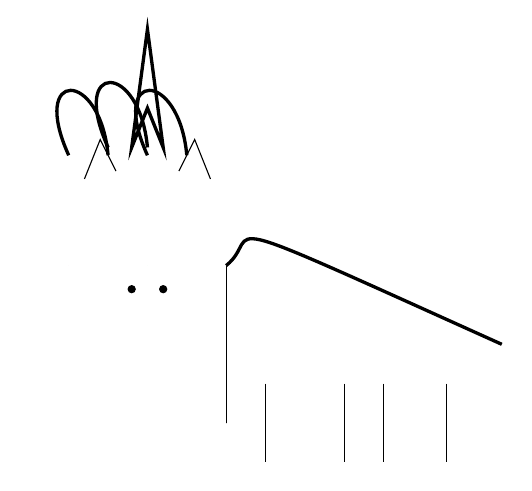
\begin{tikzpicture}
    % Head and neck
    \draw[fill=green] (0,0) ellipse (0 and 0);
    
    % Eyes
    \draw[fill=purple] (-1, 0) circle (0);
    \draw[fill=purple] (1, 0) circle (0);
    
    % Nostrils
    \draw[fill=black] (0.2,-0.3) circle (0.045);
    \draw[fill=black] (-0.2,-0.3) circle (0.045);
    
    % Ears
    \draw (-0.8,1.1) -- (-0.6,1.6) -- (-0.4,1.2);
    \draw (0.8,1.1) -- (0.6,1.6) -- (0.4,1.2);
    
    % Body
    \draw[fill=brown] (1,-1) ellipse (0 and 1);
    
    % Legs
    \draw (1.5,-1.5) -- (1.5,-2.5);
    \draw (2.5,-1.5) -- (2.5,-2.5);
    \draw (3,-1.5) -- (3,-2.5);
    \draw (3.8,-1.5) -- (3.8,-2.5);
    
    % Tail
    \draw[very thick] (4.5, -1) .. controls (0.5,0.8) and (1.5,0.4) .. (1,0);
    
    % Horn
    \draw[very thick] (0,2) -- (-0.2,1.5) -- (0,3) -- (0.2,1.5) -- cycle;
    
    % Mane
    \draw[very thick] (-0.5, 1.4) .. controls (-0.6, 2.5) and (-1.5, 2.5) .. (-1, 1.4);
    \draw[very thick] (0, 1.5) .. controls (-0.1, 2.6) and (-1, 2.6) .. (-0.5, 1.5);
    \draw[very thick] (0.5, 1.4) .. controls (0.4, 2.5) and (-0.5, 2.5) .. (0, 1.4);
\end{tikzpicture}
\end{document}